\documentclass{article}
\iffalse
This file is protected by Copyright. Please refer to the COPYRIGHT file
distributed with this source distribution.

This file is part of OpenCPI <http://www.opencpi.org>

OpenCPI is free software: you can redistribute it and/or modify it under the
terms of the GNU Lesser General Public License as published by the Free Software
Foundation, either version 3 of the License, or (at your option) any later
version.

OpenCPI is distributed in the hope that it will be useful, but WITHOUT ANY
WARRANTY; without even the implied warranty of MERCHANTABILITY or FITNESS FOR A
PARTICULAR PURPOSE. See the GNU Lesser General Public License for more details.

You should have received a copy of the GNU Lesser General Public License along
with this program. If not, see <http://www.gnu.org/licenses/>.
\fi
\author{} % Force author to be blank
%----------------------------------------------------------------------------------------
% Paper size, orientation and margins
%----------------------------------------------------------------------------------------
\usepackage{geometry}
\geometry{
	letterpaper,			% paper type
	portrait,				% text direction
	left=.75in,				% left margin
	top=.75in,				% top margin
	right=.75in,			% right margin
	bottom=.75in			% bottom margin
 }
%----------------------------------------------------------------------------------------
% Header/Footer
%----------------------------------------------------------------------------------------
\usepackage{fancyhdr} \pagestyle{fancy} % required for fancy headers
\renewcommand{\headrulewidth}{0.5pt}
\renewcommand{\footrulewidth}{0.5pt}
\rhead{\small{ANGRYVIPER Team}}
%----------------------------------------------------------------------------------------
% Appendix packages
%----------------------------------------------------------------------------------------
\usepackage[toc,page]{appendix}
%----------------------------------------------------------------------------------------
% Defined Commands & Renamed Commands
%----------------------------------------------------------------------------------------
\renewcommand{\contentsname}{Table of Contents}
\renewcommand{\listfigurename}{List of Figures}
\renewcommand{\listtablename}{List of Tables}
\newcommand{\todo}[1]{\textcolor{red}{TODO: #1}\PackageWarning{TODO:}{#1}} % To do notes
\newcommand{\code}[1]{\texttt{#1}} % For inline code snippet or command line
%----------------------------------------------------------------------------------------
% Various pacakges
%----------------------------------------------------------------------------------------
\usepackage{hyperref} % for linking urls and lists
\usepackage{graphicx} % for including pictures by file
\usepackage{listings} % for coding language styles
\usepackage{rotating} % for sideways table
\usepackage{pifont}   % for sideways table
\usepackage{pdflscape} % for landscape view
%----------------------------------------------------------------------------------------
% Table packages
%----------------------------------------------------------------------------------------
\usepackage{tabularx} % c=center,l=left,r=right,X=fill
\usepackage{float}
\floatstyle{plaintop}
\usepackage[tableposition=top]{caption}
\newcolumntype{P}[1]{>{\centering\arraybackslash}p{#1}}
\newcolumntype{M}[1]{>{\centering\arraybackslash}m{#1}}
%----------------------------------------------------------------------------------------
% Block Diagram / FSM Drawings
%----------------------------------------------------------------------------------------
\usepackage{tikz}
\usetikzlibrary{shapes,arrows,fit,positioning}
\usetikzlibrary{automata} % used for the fsm
%----------------------------------------------------------------------------------------
% Colors Used
%----------------------------------------------------------------------------------------
\usepackage{colortbl}
\definecolor{blue}{rgb}{.7,.8,.9}
\definecolor{ceruleanblue}{rgb}{0.16, 0.32, 0.75}
\definecolor{drkgreen}{rgb}{0,0.6,0}
\definecolor{deepmagenta}{rgb}{0.8, 0.0, 0.8}
\definecolor{cyan}{rgb}{0.0,0.6,0.6}
\definecolor{maroon}{rgb}{0.5,0,0}
%----------------------------------------------------------------------------------------
% Update the docTitle and docVersion per document
%----------------------------------------------------------------------------------------
\def\docTitle{Component Data Sheet}
\def\docVersion{1.5}
%----------------------------------------------------------------------------------------
\date{Version \docVersion} % Force date to be blank and override date with version
\title{\docTitle}
\lhead{\small{\docTitle}}

\def\comp{device\_name}
\def\Comp{Device Name}
\graphicspath{ {figures/} }

\begin{document}

\section*{Summary - \Comp}
\begin{tabular}{|c|M{13.5cm}|}
	\hline
	\rowcolor{blue}
	•               & •                                 \\
	\hline
	Name              & \comp                               \\
	\hline
	Worker Type       & Device                              \\
	\hline
	Version           & v\docVersion                               \\
	\hline
	Release Date      & 4/2019                        \\
	\hline
	Component Library & Name of component library           \\
	\hline
	Workers           & Names of all worker implementations \\
	\hline
	Tested Platforms  & List of tested platforms            \\
	\hline
\end{tabular}

\section*{Functionality}
\begin{flushleft}
	A description of the component's functionality
\end{flushleft}

\section*{Worker Implementation Details}
\begin{flushleft}
	For each worker implementation, a short description of the implementation specific features
	\subsection*{\comp.rcc}
	\subsection*{\comp.hdl}
\end{flushleft}

\section*{Theory}
\begin{flushleft}
	Any theoretical discussion of component's operation.
\end{flushleft}

\section*{Block Diagrams}
\subsection*{Top level}
\begin{center}
	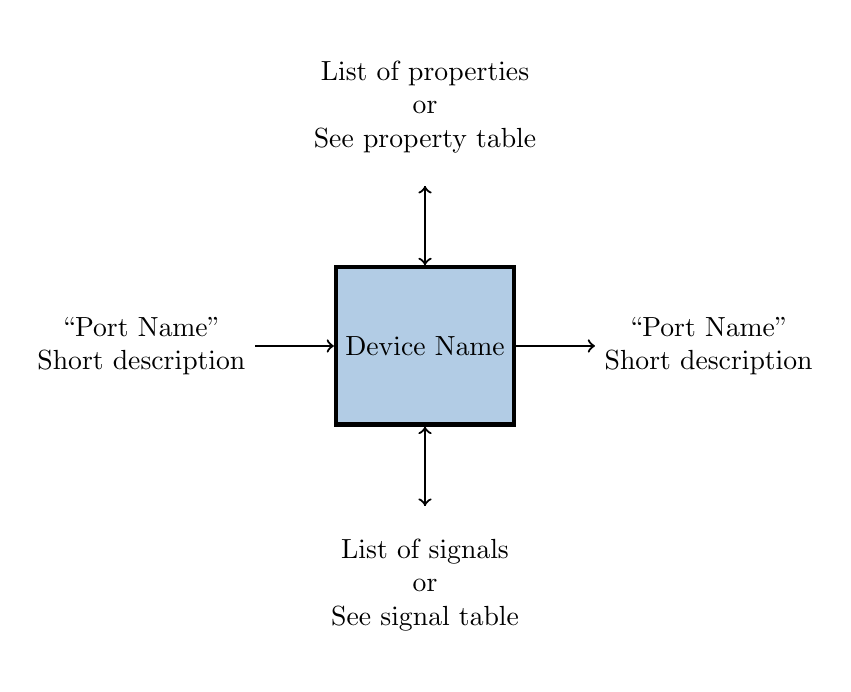
\begin{tikzpicture}[% List of styles applied to all, to override specify on a case-by-case
			every node/.style={
				align=center,  		% use this so that the "\\" for line break works
				minimum size=2cm	% creates space above and below text in rectangle
			},
			every edge/.style={draw,thick}
		]
		\node[rectangle,ultra thick,draw=black,fill=blue](R2){\Comp};
		\node[rectangle,draw=white,fill=white](R3)[left= of R2]{``Port Name'' \\ Short description};
		\node[rectangle,draw=white,fill=white](R4)[right= of R2]{``Port Name'' \\ Short description};
		\node[rectangle,draw=white,fill=white](R5)[above= of R2]{List of properties\\ or\\ See property table};
		\node[rectangle,draw=white,fill=white](R6)[below= of R2]{List of signals\\ or\\ See signal table};
		\path[->]
		(R3)edge []	node [] {} (R2)
		(R2)edge []	node [] {} (R4)
		(R2)edge []	node [] {} (R5)
		(R5)edge []	node [] {} (R2)
		(R2)edge []	node [] {} (R6)
		(R6)edge []	node [] {} (R2)
		;
	\end{tikzpicture}
\end{center}

\subsection*{State Machine}
If applicable, include a state diagram of any state machine used

\section*{Source Dependencies}
For each worker implementation, list 3rd party or local source or library dependencies
\subsection*{\comp.rcc}
\subsection*{\comp.hdl}

\begin{landscape}
	\section*{Component Spec Properties}
	\begin{scriptsize}
		\begin{tabular}{|p{3cm}|p{1.5cm}|c|c|c|c|c|p{7cm}|}
			\hline
			\rowcolor{blue}
			Name & Type & SequenceLength & ArrayDimensions & Accessibility & Valid Range & Default & Usage \\
			\hline
			     &      &                &                 &               &             &         &       \\
			\hline
		\end{tabular}
	\end{scriptsize}

	\section*{Worker Properties}
	\subsection*{\comp.hdl}
	\begin{scriptsize}
		\begin{tabular}{|p{3cm}|p{2cm}|p{1cm}|c|c|c|c|c|p{5cm}|}
			\hline
			\rowcolor{blue}
			Type & Name & Type & SequenceLength & ArrayDimensions & Accessibility & Valid Range & Default & Usage \\
			\hline
			Property/SpecProperty & & & & & & &\\
			\hline
		\end{tabular}
	\end{scriptsize}

	\section*{Component Ports}
	\begin{scriptsize}
		\begin{tabular}{|M{2cm}|M{1.5cm}|M{4cm}|c|c|M{9cm}|}
			\hline
			\rowcolor{blue}
			Name & Producer & Protocol & Optional & Advanced & Usage \\
			\hline
			& & & &\\
			\hline
		\end{tabular}
	\end{scriptsize}

	\section*{Worker Interfaces}
	\subsection*{\comp.hdl}
	\begin{scriptsize}
		\begin{tabular}{|M{2cm}|M{1.5cm}|c|c|M{12cm}|}
			\hline
			\rowcolor{blue}
			Type & Name & DataWidth & Advanced & Usage \\
			\hline
			& & &\\
			\hline
		\end{tabular}
	\end{scriptsize}

	\section*{Signals}
	\begin{scriptsize}
		\begin{tabular}{|M{2.5cm}|M{1.5cm}|M{1.5cm}|M{14.5cm}|}
			\hline
			\rowcolor{blue}
			Name & Type & Width & Description \\
			\hline
			     &      &       &             \\
			\hline
		\end{tabular}
	\end{scriptsize}

\end{landscape}

\section*{Control Timing and Signals}
\begin{flushleft}
	An HDL worker only section. For any RCC only worker implementations, this section can be removed.
\end{flushleft}

\section*{Performance and Resource Utilization}
For each worker implementation, list utilization statistics for relevant parameter sets for each implementation.
\subsubsection*{\comp.rcc}
\begin{scriptsize}
	\begin{tabular}{|c|c|c|}
		\hline
		\rowcolor{blue}
		Processor Type & Processor Frequency & Run Function Time \\
		\hline
		               &                     &                   \\
		\hline
	\end{tabular}
\end{scriptsize}

\subsubsection*{\comp.hdl}
\begin{scriptsize}
	\begin{tabular}{|c|c|c|c|c|c|c|c|}
		\hline
		\rowcolor{blue}
		Device & Registers & LUTs & Fmax & Memory/Special Functions & GCLK & I/O & Design Suite \\
		\hline
		       &           &      &      &                          &      &     &              \\
		\hline
	\end{tabular}
\end{scriptsize}

\section*{Test and Verification}
\begin{flushleft}
	Description of test methodology for worker including details of input data generation and output data validation, instructions of how to run the test, and expected results. Ensure worker implementation specific test conditions/results are indicated here.
\end{flushleft}
\section*{References}
\begin{flushleft}
\end{flushleft}
\end{document}
